%Tex-Stuff
\documentclass[a4paper,12pt]{article}

%Imports
\usepackage[pdftex]{graphicx}
\usepackage[utf8]{inputenc}
\usepackage{subcaption}
\usepackage{hyperref}


%%%%%%%%%%%%%%%%%%%%%%%%%%%%%%%%%%%%%%%%%%%%%%%%
\begin{document}

\section{PaperOverflow: Produktivision}
Die Beschreibung der Produktvision erfolgt noch den Feldern des  \href{http://www.romanpichler.com/tools/vision-board/}{"Product-Vision-Boards"} von Roman Pichler. 
\begin{figure}[h!]
  \centering
  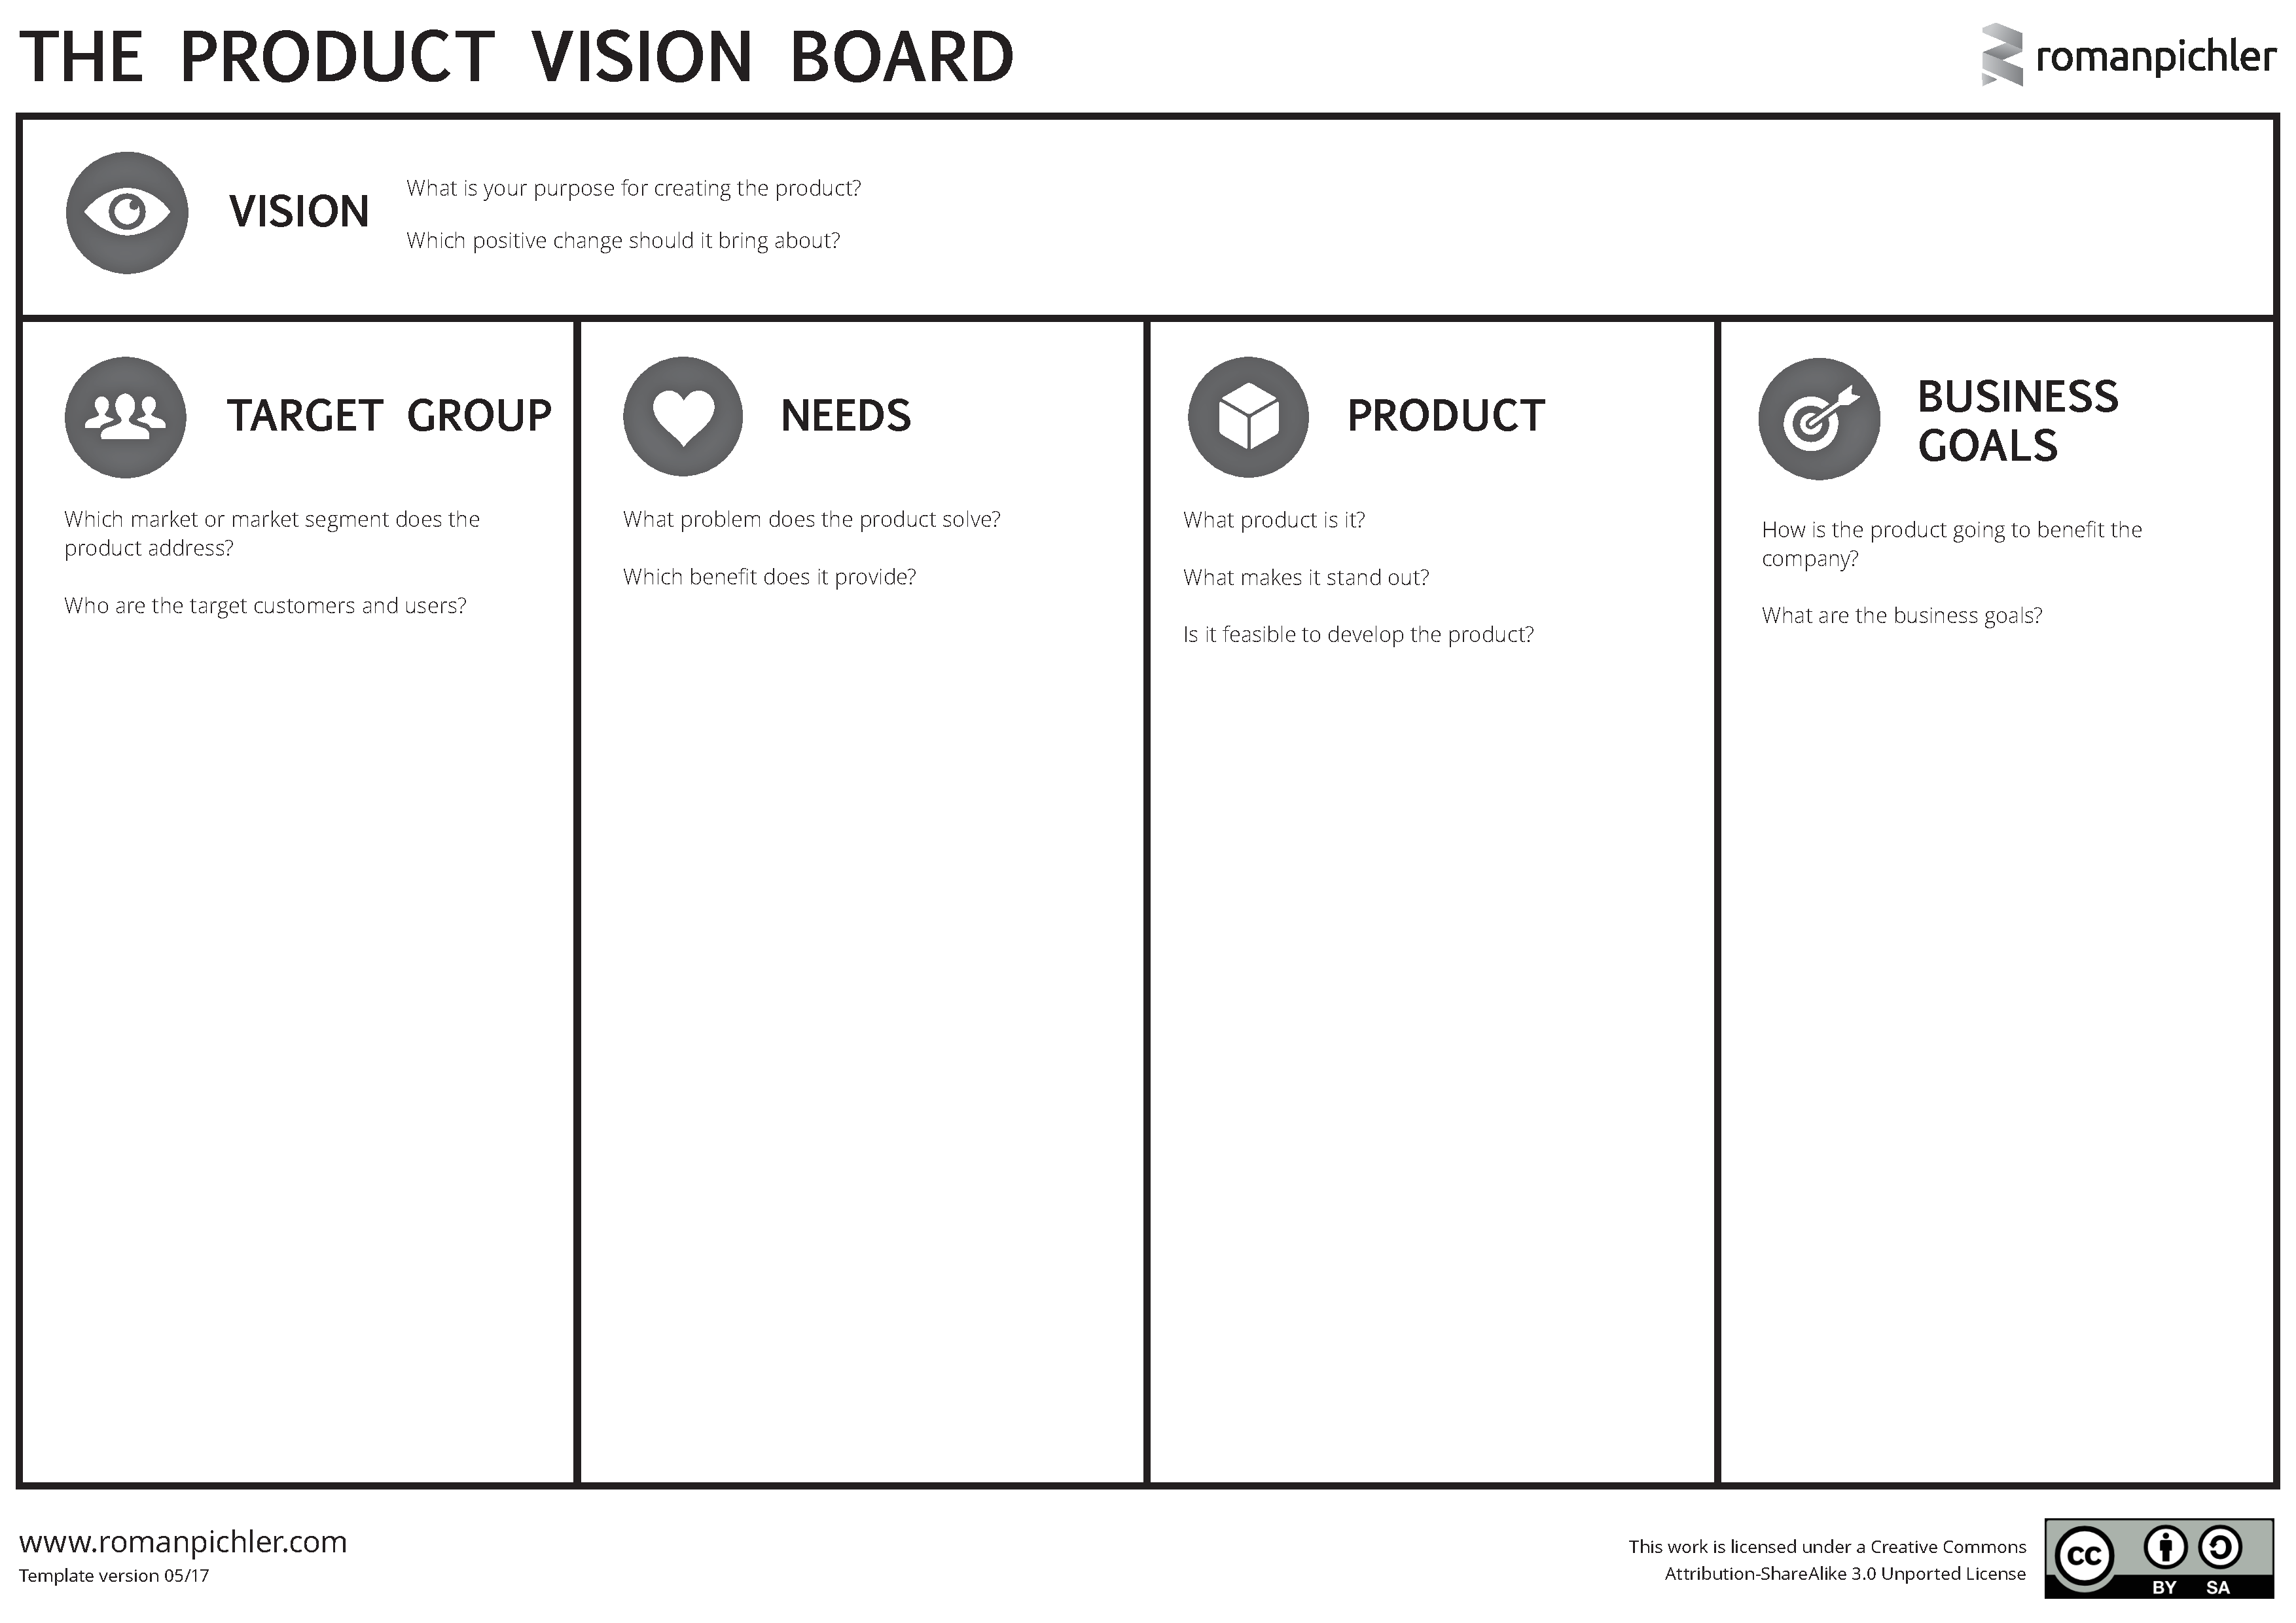
\includegraphics[width=0.7\linewidth]{res/PVB.pdf}
\end{figure}

Besonderes Augenmerk soll dabei auf die Produktbeschreibung gelegt werden.
Die Geschäfts-Ziele hingegen, sollen aufgrund der geringen Relevanz für das Projekt nicht beleuchtet werden.

\subsection{Vision}
Ziel von PaperOverflow ist es den Autoren von wissenschaftlichen Arbeiten im Bereich der Literaturverwaltung zu unterstützen. Dabei soll die PaperOverflow im Gegensatz zu ähnlichen Produkten komfortabel und unkompliziert sein, fehlerhafte Zitate vermeiden, ein Aufsuchen von zitierbaren Textstellen ermöglichen und mit wachsender Menge an zu verwaltenden Dokumenten besser werden.

\subsection{Zielgruppe}
Wer sind die Anwender von PaperOverflow?\\
Zunächst wird PaperOverflow von Benutzern verwendet, deren Ziel es ist eine wissenschaftliche Arbeit zu verfassen. PaperOverflow soll für diese Benutzer die Verwaltung von wissenschaftlichen Veröffentlichungen anderer Autoren übernehmen.\\
Vorrangig soll das Auditorium von PaperOverflow aus Anwendern bestehen, welche zum Verfassen der Wissenschaftlichen Arbeit LaTeX verwenden. Jedoch sollen auch Nicht-LaTeX-Benutzer PaperOverflow zur Verwaltung von Veröffentlichungen nutzen können.\\
PaperOverflow soll zum einen von Benutzern verwendet werden, die technisch versiert sind und gerne mit komplexer wirkenden, dafür jedoch mächtigeren Oberflächen arbeiten. Zum anderen sollen auch weniger technisch versierte Nutzer durch eine einfache Oberfläche angenehm mit PaperOverflow arbeiten können.\\
Des Weiteren werden die Anwender von PaperOverflow verscheiden große Mengen an Veröffentlichungen zu verwalten haben. Dabei soll sich der Einsatz der Software schon ab wenigen Dokumenten lohnen, aber auch riesige Mengen an Veröffentlichungen handhaben können. Das Verhältnis, welche Dokumente in digitaler Form vorliegen und welche als haptisches Exemplar vorhanden sind, variiert dabei ebenfalls von Nutzer zu Nutzer.\\
\\
Um die oben genannten variierenden Eigenschaften der Zielgruppe zu veranschaulichen, sollen als Vertreter der gesamten Zielgruppe drei Personas aufgelistet werden.

\paragraph{Wolfgang der Word-User mit wenigen Dokumenten}
- Wolfgang möchte einen kurzen wissenschaftlichen Artikel veröffentlichen und hat sich entscheiden dies in Microsoft Word zu tun. Er benötigt nur eine Hand voll wissenschaftlicher Quellen, die er richtig zitiert. Diese Quellen liegen ihm teils digital, teils analog vor. Er ist nicht weiter technisch versiert und es ist auch nicht zu erwarten, dass er in näherer Zeit weitere wissenschaftliche Arbeiten schreiben wird.

\paragraph{Larissa die LaTeX-Userin mit vorrangig digitalen Dokumenten}
- Larissa nutzt LaTeX, um ihre Abschlussarbeit anzufertigen. Sie setzt sich dafür zum ersten Mal intensiver mit LaTeX und BibTeX auseinander. Sie hat für Ihre Arbeit etwa 40 potentielle Quellen, von denen Sie voraussichtlich etwa 30 zitieren wird. Die Quellen liegen Larissa hauptsächlich in digitaler Form vor.

\paragraph{Prof. Probst der LaTeX-Power-User mit vorrangig analogen Dokumenten}
- Prof. Probst ist LaTeX-Vollprofi und verfasst regelmäßig wissenschaftliche Dokuemnte zu verschiedenen Themen und verschiedenen Fachrichtungen. Er hat inzwischen eine Dokumentensammlung von 1200 wissenschaftlichen Veröffentlichungen. Davon stehen die meisten in seinem Bücherregal, nur wenige liegen ihm in digitaler Form vor.

\subsection{Bedürfnisse}

Alle drei oben genannten Persona haben generell das Bedürfnis Literatur in digitaler oder analoger Form einfach und unkompliziert als Ressource zu erfassen, in den erfassten Ressourcen komfortabel nach Inhalten suchen zu können und die benötigten Textstellen mit wenigen Klicks korrekt und dem verwendetem Ziteirstandard entsprechend zu ziteren.\\

Dabei steht für Persona Wolfgang vor allem die Einfachheit aller Schritte im Vorderugrund. Für diesen Nutzer müssen vor allem simple Möglichkeiten für das schnelle Zitieren und eine ansprechende, simple Benutzeroberfläche gegeben sein. Die Operationen um Literatur zu erfassen, Zitate zu finden und diese korrekt zu zitieren müssen für Wolfgang auf ein Minimum reduziert werden können.\\

Für Persona Larissa liegt das besondere Augenmerk auf dem einfachen und komfortablen Hinzufügen von wissenschaftlichen Dokumenten im PDF sowie dem komfortablen zitieren von Stellen in diesen Dokumenten. Die gefundenen Zitate sollen in einem Set zusammengefasst werden, welches im BibTeX-Format exportiert werden soll. Larissa benötigt eine größere BibTeX-Datei, welche alle zu zitierenden Stellen enthält. Diese Stellen soll Sie innerhalb des LaTeX-Dokuments referenzieren können.\\

Persona Prof. Probst benötigt vor allem eine Möglichkeit seine 1000 analog vorliegenden wissenschaftlichen Dokumente schnell und einfach im PaperOverflow zu erfassen. Besonders ist dabei eine Unterstützung beim Hinzufügen von Stichworten zu den Dokuemnten benötigt, um später möglichst genaue Treffer bei der Suche zu erhalten. Beim Erfassen ist zusätzlich eine Unterteilung der erfassten Dokumente in Kategorien notwendig, um später die Suche genauer eingrenzen zu können. Beispielsweise ist eine solche Unterteilung nach Themengebiet benötiogt, wenn Prof. Probst in zwei verscheidenen Fachbereichen arbeitet und die Dokumente des einen Fachbreriches keine Relevanz für den anderen haben. Eine Zuordnung zu Kategorien möchte der Prof. sowohl beim Import als auch im Nachgang vornehmen können. \\
Beim Suchen von Dokumenten benötigt Prof. Probst sowohl eine Kategorie-spezifische Suche, als auch eine Suche in der kompletten Menge der erfassten Dokumente. Für Prof. Probst als technisch versierten Benutzer mit vielen Dokumenten soll eine erweiterte Suche möglich sein, durch die sich Suchanfragen genauer spezifizieren lassen.\\
Ist ein Dokument gefunden, benötigt Prof. Probst Empfehlungen, welche weiteren Dokuemnte, die sich im PaperOverflow befinden, für Ihn von Interesse sein können.\\
Für das Zitieren benötigt Prof. Probst analog zu Persona Larissa eine Möglichkeit Zitate zu einem Set zusammenzufassen und später als BibTeX-Datei zu exportieren. Dabie benötigt Prof. Probst mehrere verschiedene Sets an Zitaten, für den Fall dass er an mehreren Arbeiten arbeitet. Die Kategorisierung der Sets solll dabei durch Prof. Probst konfigurabel sein.

\subsection{Produktbeschreibung}

Sie haben sich dazu entschieden eine wissenschaftliche Arbeit zu verfassen und sind nun dabei sich Wissen zum Themengebiet heranzuziehen? Und der Haufen der Veröffentlichungen wir immer größer und größer? Und ganz allmählich unbezwingbar? Sie nähern sich langsam der Grenze, ab der sie einfach nicht mehr Dokumente handhaben können? Dem Overflow an Papers? 
\begin{center}
Keine Panik! 
\end{center}
Der Overflow ist nicht böse, er braucht nur die richtige Handhabe. Mit PaperOverflow holen Sie das Maximum aus Ihrer Dokumentensammlung heraus!\\ \\
PaperOverflow unterstützt Sie in Ihrem Arbeiten, in den drei folgenden Schritten:

\renewcommand\thesubfigure{\arabic{subfigure}}
\begin{figure}[h!]
  \centering
  \begin{subfigure}[b]{0.32\linewidth}
    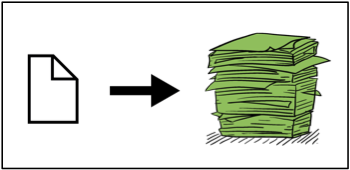
\includegraphics[width=\linewidth]{res/step1.png}
    \caption{Den PaperOverflow nähren.}
    %\label{fig:1} 
  \end{subfigure}
  \begin{subfigure}[b]{0.32\linewidth}
    
\includegraphics[width=\linewidth]{res/step2.png}
    \caption{Den PaperOverflow durchsuchen}
    %\label{fig:2} 
  \end{subfigure}
  \begin{subfigure}[b]{0.32\linewidth}
    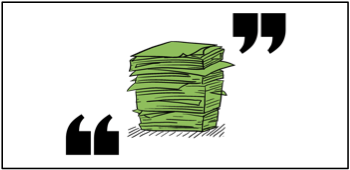
\includegraphics[width=\linewidth]{res/step3.png}
    \caption{Den PaperOverflow zitieren}
    %\label{fig:3} 
  \end{subfigure}
\end{figure}



\paragraph{Den PaperOverflow nähren.}\

PaperOverflow unterstützt Sie bei dem Erfassen Ihrer Dokumente. \\

\textbf{Dokumente in gedruckter Form:} 
\begin{itemize}
	\item Holen Sie das Dokument aus dem Schrank
	\item Erfassen Sie über die ISBN-Nummer, den Titel oder den Autor mit Unterstützung einer Auto-Vervollständigung Ihr Dokument als Paper.
	\item PaperOverflow bietet Ihnen Vorschläge an, um welches Dokument es sich handelt. Wählen Sie eine Alternative und bestätigen Sie. 
	\item Eine manuelle Korrektur oder Vervollständigung der Daten ist jederzeit möglich.
	\item PaperOverflow schlägt Ihnen Stichworte für den Dokumenteninhalt an. Diese sind für die spätere Suche nach Papers nützlich. Wählen sie passende Stichworte aus oder fügen Sie komfortabel weitere hinzu.
	\item Mit wenigen Klicks ist damit Ihr Dokument als Paper dem PaperOverfolw hinzugefügt.
	\item Oder importieren Sie fertige Meta-Daten \textit{(BibTex, BibX, RIS, PubMed)}
\end{itemize} \

\textbf{Dokument als Datei:}
\begin{itemize}
	\item Legen Sie das Dokument per Drag and Drop im PaperOverflow als Paper ab.
	\item Sobald Sie das Dokument abgelegt haben holt PaperOverflow für Sie die Meta-Informationen und bietet Ihnen einen Vorschlag an, um welches Dokument es sich handelt. Bestätigen Sie oder wählen Sie ggf. eine Alternative.
	\item Eine manuelle Korrektur oder Vervollständigung der Daten ist jederzeit möglich.
	\item PaperOverflow sucht Ihnen die Stichworte für den Dokumenteninhalt aus dem Dokument und bietet diese Als Vorschlag an. Wählen sie passende Stichworte aus oder fügen Sie komfortabel weitere hinzu.
	\item Ist das Dokument als Paper im PaperOverflow abgelegt, Können Sie es später jederzeit als Datei exportieren.
\end{itemize}\ 

\textbf{Ihr PaperOverflow wird groß? $\to$ Nutzen Sie PaperStacks!}
\begin{itemize}
	\item Ordnung von Beginn an: Legen Sie für Ihre Dokumente verscheidene PaperStacks an! Damit lassen sich Papers für gänzlich verschiedene Themenbereich von Beginn an voneinander abtrennen.
	\item Schon beim Zufügen von Papers zum PaperOverflow ist das Zuordnen von Papers zu einem bestimmten PaperStack möglich.
	\item Eine Bearbeitung der Zuordnung von Papers zu PaperStacks ist jederzeit möglich.
\end{itemize}

\paragraph{Den PaperOverflow durchsuchen}\ 

Sie haben Ihre Papers im PaperOverflow erfasst? Starten Sie mit der Recherche und suchen Sie nun im PaperOverflow nach guten Zitaten!

\begin{itemize}
	\item Suchen Sie komfortabel nach Stichworten, Titeln, Autoren und Inhalten von Abstracts.
	\item Lassen Sie sich durch Auto-Vervollständigung bei Suchanfragen unterstützen.
	\item Sie wollen es genau wissen? Nutzen Sie die erweiterte Suchfunktion und präzisieren Sie Ihre Suchanfrage genauestens.
	\item Blicke Sie zurück: PaperOverflow bietet Ihnen die Möglichkeit Ihre Suchanfragen zu historisieren.
	\item Die haben ein Paper vor Augen? Erhalten Sie Vorschläge für ähnliche Papers!
	\item Das Dokument liegt digital vor? Zeigen Sie es an und lesen Sie rein!
\end{itemize}

\paragraph{Den PaperOverflow zitieren}\ 

Sie haben ein passendes Zitat im Paper gefunden? Zitieren Sie nun den PaperOverflow!\\

Für Papers, die im PaperOverflow in digitaler Form vorliegen lässt sich die entsprechende Stelle markieren und per Knopfdruck zitieren. Ein entsprechendes Quote wird erstellt und die Seitenzahl autmatisch hinzugefügt.\\
Für Papers in analoger Form lassen sich ebenfalls unter Angebe der Seitenzahl in zwei Klicks Quotes erstellen.\\
Jedem Quote können Sie eine Bemerkung anfügen, was das Zitat enthält oder weshalb und wo Sie es einsetzen möchten.\\

\textbf{QuickQuote und QuoteSets!}
\begin{itemize}
	\item Sie möchten nur kurz eine Stelle markieren? Nutzen Sie QuickQuote! Mit einem Klick haben Sie die entsprechende Stelle als BibTeX oder als Quellenangabe in der Zwischenablage und können Sie weiterverarbeiten.
	\item Sie brauchen mehrere Zitate? Fügen Sie Ihre Zitate mit einer kurzen Bemerkung zu Ihrer QuoteCollection hinzu und suchen Sie weiter.
	\item Sie haben mehr als eine Arbeit, für die Sie zitate sammeln? Organisieren Sie Ihre Quotes in QuoteSets! QuoteSets gruppieren Quotes und sind durch den Benutzer konfigurierbar.
\end{itemize}

\textbf{Export als BibTeX oder Referenzliste}\\
Exportieren Sie Ihre Quotes Zitierstandard-konform \textit{(APA, Chicago/Turabian, Harvard, MLA, Flexibel Einstellbares CustomFormat)}
\begin{itemize}
	\item Exportieren Sie Ihre QuoteCollection oder einzelne QuoteSets in den gängigen Exportformaten. \textit{(BibTex, RIS, BibX)}
	\item Oder Export Sie Ihre QuoteCollection oder einzelne QuoteSets als Referenzlisten \textit{(HTML, RTF, reiner Text, PDF)}
	\item Sie arbeiten mit anderen Personen gemeinsam? Treten Sie in Kontakt! Senden Sie Ihre Zitate per Mail Ihren Co-Autoren zu.
\end{itemize}



\pagebreak
\section{PaperOverflow: Vokabeln}
\begin{tabular}{ p{5cm} p{8.5cm} }
  \textbf{Analoges Paper} & Paper zu denen ein gedrucktes wissenschaftliches Domument vorliegt. \\ \\
  \textbf{Digitales Paper} & Paper zu denen eine PDF-Datei vorliegt. \\ \\
  \textbf{Paper} & Das zum PaperOverflow hinzugefügte wissenschaftliche Dokument. Dieses enthält im Falle eines analogen Papers nur die Metadaten oder im Falle eines digitalen Papers die Metadaten und zusätzlich die PDF-Datei. \\ \\
  \textbf{PaperOverflow} & Zum einen das Programm selbst. Zum anderen bezeichnet der PaperOverflow den alle Papers im Programm (alle im Programm erfassten Dokumente) \\ \\
  \textbf{PaperStack} & Bezeichnet einen Teil des PaperOverflows. Also nur einen kleinen Stapel an Papers. Verscheidene PaperStack können genutzt werden, um Dokumente verschiedener Kategorien voneinander abzutrennen.\\ \\
  \textbf{Quote} & Eine zitierte Stelle wird als Quote gespeichert.\\ \\
  \textbf{QuoteSet} & Mehrere Quotes lassen sich zu einem Set an Quotes, einem QuoteSet, zusammenfassen.\\ \\
  \textbf{QuoteCollection} & Umfasst all Ihre QuoteSets und Quotes
\end{tabular}



\end{document}
%%%%%%%%%%%%%%%%%%%%%%%%%%%%%%%%%%%%%%%%%%%%%%%%